Tato kapitola je věnována realizaci navrhovaného systému. Kapitola je rozdělena na dvě podkapitoly a to na implementaci a testování.

V části zaměřené na implementaci jsou popsány použité technologie, je představena struktura jednotlivých modulů a jsou zde popsány jednotlivá rozhraní, třídy a pohledy. Další částí v této podkapitole jsou implementační poznámky, kde jsou popsány použité knihovny a řešení autentizace a autorizace.

V druhé části zaměřené na testování je popsán průběh testování systému a výsledky testování.

\section{Implementace}

\subsection{Použité technologie}
Vyvíjený informační systém lze rozdělit na tři dílčí části. První částí je backend aplikace. To je část, která se stará o logiku aplikace, plnění funkcí systému a zpracovávání procesů. Druhou částí je frontend, ten se stará o vzhled aplikace. Je to část systému, se kterou pracuje koncový uživatel. Poslední částí je databáze, kam se ukládají potřebná data.

\subsubsection{Backend}
Backend systému je vyvíjen na platformě .NET Core s použitím jazyka C\# a ASP.NET Core MVC frameworku. Volba platformy .NET Core je dána ze zadání práce.

.NET Core je open-source platforma vyvíjená a podporovaná společností Microsoft. V rámci této platformy lze vyvíjet webové, desktopové, konzolové či mobilní aplikace, programy pro IoT a další. Aplikace lze vyvíjet pro velkou škálu operačních systémů, nejen pro Microsoft Windows. Lze vytvářet programy i pro operační systém Linux, macOS, Android, iOS a další. Aplikace mohou být i multiplatformní, což znamená, že jedna aplikace může být spuštěna na vícero různých operačních systémech. \cite{net-introduction} 

ASP.NET Core MVC je open-source framework pro tvorbu webových aplikací na platformě .NET Core. Tento framework poskytuje programátorovi zázemí pro vytváření aplikací s MVC architekturou. Obsahuje mimo jiné i systém pro routování, který umožňuje programátorovi definovat, jakým způsobem se budou zpracovávat URL adresy, systém pro binding modelů, který umožňuje předávat objekty do HTML šablon, a vestavěnou podporu pro dependency injection \cite{net-mvc-overview}, což je návrhový vzor k dosažení IoC (Inversion of Control) mezi třídami a jejich závislostmi \cite{net-dependency-injection}. V ASP.NET Core MVC se závislosti předávají do třídy pomocí konstruktoru, jehož parametry tvoří vkládané závislosti (rozhraní). Konkrétní implementace, které budou nakonec použity a jakým způsobem se vytvoří, se určí ve třídě \texttt{Startup.cs}. Programy v tomto frameworku mohou být vyvíjeny a provozovány v operačních systémech Microsoft Windows, Linux i macOS \cite{net-core-introduction}.

Zdrojový kód je napsán v jazyce C\#, což je objektově orientovaný a typově bezpečný programovací jazyk od společnosti Microsoft.

Backend aplikace se na rozdíl od frontend části vyznačuje tím, že je provozován na serveru, na který poté přichází požadavky od klienta. Požadavek může chtít vrátit celou webovou stránku, určitá data a jiné. Ve vyvíjeném systému požadavek typicky žádá o webovou stránku. Celý proces začíná tím, že klient pošle požadavek na server s cílem získat určitou webovou stránku. Server zavolá ASP.NET Core, který podle URL adresy pozná, co klient požaduje. V případě potřeby si program zajistí data a poté, pomocí vytvořených šablon, sestaví webovou stránku, kterou pošle klientovi zpět.

\subsubsection{Frontend}
Frontend je primárně vytvořen pomocí HTML šablon, které se používají při vývoji ASP.NET Core MVC aplikací, a doplněn jazykem CSS, Bootstrap frameworkem a JavaScriptem. 
V návrhovém vzoru MVC (model-view-controller) se HTML šablony nachází ve view vrstvě (vrstvě pohledů). Každá šablona představuje webovou stránku nebo její část. Tato šablona může obsahovat HTML nebo C\# kód, ten je do šablon vkládán pomocí značkovacího jazyka Razor. Tyto šablony lze poznat podle toho, že mají příponu \texttt{.cshtml}. \cite{net-views}

CSS (Cascading Style Sheets) je jazyk, pomocí kterého se definují styly HTML elementů. Popisuje se s ním například layout stránky, barva a velikost elementu, apod. Lze s nimi také popisovat HTML elementy na základě velikosti obrazovky zařízení. \cite{css}

Bootstrap je bezplatný, open-source framework, který usnadňuje vývoj frontend části webových stránek. Obsahuje velké množství předpřipravených HTML a CSS komponent, například tlačítka, tabulky, navigační panely a další. Framework také umožňuje programátorovi jednoduše řešit problém responzivity webových stránek (zobrazení na zařízeních s různou velikostí displeje). V tomto projektu Bootstrap pomohl jak se vzhledem stránky, tak při řešení responzivity. Oproti konkurenčním projektům nabízí především větší uživatelskou základnu, jedná se totiž o nejpopulárnější framework svého druhu. \cite{bootstrap-w3s, bootstrap}

Posledním použitým nástrojem je JavaScript resp. jQuery \cite{jquery}. JavaScript je skriptovací jazyk, který umožňuje vytvářet dynamický obsah na webových stránkách, a to u klienta ve webovém prohlížeči \cite{what-is-js}. Lze ho použít například pro uložení nějaké informace do proměnné či reagovat na nějakou akci, kterou uživatel provede \cite{what-is-js}. jQuery je knihovna napsaná v JavaScriptu, která usnadňuje práci se zpracováním událostí, manipulací obsahu HTML stránky a další. Tyto technologie využívá v projektu především Bootstrap framework, využity byly také při zobrazování postranního navigačního panelu u zařízení s menším displejem. Hlavním důvodem použití jQuery oproti alternativám (např. React \cite{react}) byl fakt, že tuto knihovnu již využívá Bootstrap framework. Navíc knihovna byla použita pro řešení velmi jednoduchých problémů typických právě pro jQuery.

Frontend aplikace je provozován na straně klienta, odkud jsou poté přechodem na jinou URL adresu posílány požadavky na server.

\subsubsection{Databáze}
Pro uchovávání dat, se kterými aplikace pracují se využívají databáze. Ty se dělí na několik druhů, například relační, nerelační (NoSQL), grafové, distribuované a další. Výběr typu databáze záleží na tom, jakým způsobem budou data používána. Například NoSQL se používá pro ukládání nestrukturovaných dat nebo dat, nad kterými se budou provádět složité vyhledávací operace. Pro aplikaci vyvíjenou v rámci této práce byla z důvodu nutnosti integrity dat a faktu, že data mají mezi sebou jasně definované vztahy, zvolena relační databáze, která je pro tyto omezení vhodná. \cite{co-je-sql, sql-vs-nosql}

Pro vývoj databáze byl použit Entity Framework Core s code-first přístupem. Entity Framework Core je ORM framework, který umožňuje vývojáři pracovat s tabulkami databáze jako s objekty. Umožňuje mapovat třídy jako tabulky databáze, provádět SQL příkazy pomocí LINQ (Language Integrated Query) či ukládat data do databáze. Pro přístup k datům je nejprve nutné definovat tzv. model, ten je tvořen entitními třídami a databázovým kontextem. Model mapuje entity a vztahy na tabulky v databázi. Databázový kontext je objekt, který udržuje relaci s databází a probíhají pomocí něj dotazy do databáze či ukládání dat \cite{ef-core}. V aplikaci to vypadá tak, že pro tabulku je vytvořena třída, která obsahuje vlastnosti (property), které odpovídají sloupcům v tabulce. V třídě databázového kontextu poté lze třídám/tabulkám přiřazovat různé vztahy a vlastnosti, například cizí klíče, informaci, jestli může být sloupec prázdný, apod. Databázový kontext dále obsahuje informace o použité databázi a kolekce entitních tříd, které obsahují všechny dostupné entity (záznamy) daného typu.

Code-first přístup je technika, která umožňuje vytvořit a udržovat databázi a její tabulky pomocí zdrojového kódu na platformě .NET Core \cite{code-first}. Znamená to tedy, že databáze ani tabulky se nevytváří a neupravují pomocí SQL skriptů ručně, ale všechny vlastnosti a vztahy mezi tabulkami se definují v entitních třídách a databázovém kontextu. Vytváření a přenos změn v databázi poté zajišťuje Entity Framework Core pomocí tzv. migrací, které převedou definovaný zdrojový kód do databáze/tabulek. Entity Framework Core nabízí kromě code-first ještě jeden další přístup. Tím je databázový přístup. Ten spočívá v tom, že databáze již existuje nebo je vytvořena samostatně. Entity Framework Core poté vytvoří model (entitní třídy a databázový kontext) podle tabulek v databázi \cite{ef-core}. Výhodou code-first přístupu je, že není potřeba využívat další nástroj pro tvorbu schématu databáze, všechny změny, které se pomocí migrace dostanou do databáze, jsou sledovány a mohou být snadno vráceny zpět. Vývojář má také kontrolu nad tím, jak databáze vypadá a funguje, protože se vyhne automaticky generovanému kódu. Z těchto důvodů byl pro vyvíjený systém zvolen code-first přístup.

Entity Framework Core umí pracovat s celou řadou databází pomocí stažitelných knihoven. Dokáže pracovat například s Microsoft SQL Server 2012 a novější, SQLite 3.7 a novější, PostgreSQL, MySQL, Oracle DB a další \cite{database-providers}. Při vývoji byla použita databáze Microsoft SQL Server. Aplikace je připravena na provoz jak s Microsoft SQL Server, tak s PostgreSQL databází. Podpora obou těchto databází poskytuje větší možnosti školám při provozu aplikace. Postup, jak aplikaci nasadit, je popsán v instalační příručce, která je součástí přílohy této práce.

\subsection{Prezentační vrstva}
Prezentační vrstva je rozdělena do tzv. oblastí (areas), ty umožňují rozdělit zdrojový kód v ASP.NET Core MVC aplikaci do menších funkčních celků \cite{areas}. Každý modul, kromě základního modulu Base, má vlastní oblast. Zdrojový kód Base modulu je umístěn v root adresáři projektu. Každý modul je podle návrhu rozdělen na modely, pohledy a kontrolery. Strukturu projektu pro prezentační vrstvu můžeme vidět na obrázku \ref{struktura-projektu}.
\clearpage

\begin{figure}[h]
	\centering
	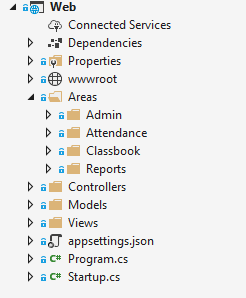
\includegraphics[width=0.5\textwidth]{images/struktura_projektu.png}
	\caption{Struktura projektu prezentační vrstvy}
	\label{struktura-projektu}
\end{figure}

\subsubsection{Základní modul -- Base}
Základní modul je umístěn v root adresáři projektu Web. Modul obsahuje tyto kontrolery:
\begin{itemize}
    \item \texttt{AccountController}
    \begin{itemize}
        \item Kontroler slouží pro obecnou práci s uživateli. Umožňuje uživateli přihlášení do systému, odhlášení, změnu hesla a zobrazení základních informací o účtu. Práce s tímto kontrolerem není omezena na žádnou roli uživatele, některé metody však požadují přihlášeného uživatele.
    \end{itemize}
    \item \texttt{HomeController}
    \begin{itemize}
        \item Úlohou tohoto kontroleru je přesměrování přihlášeného uživatele na jeho domovskou stránku. Například rodiče přesměruje na stránku s rychlým přehledem o jeho dětech, admina přesměruje na stránku, kde se provádí administrace. Tento kontroler požaduje přihlášeného uživatele.
    \end{itemize}
\end{itemize}

\clearpage
Přehled pohledů podle kontrolerů:

\begin{itemize}
    \item \texttt{AccountController}
    \begin{itemize}
        \item \texttt{AccessDenied} -- V případě odepření přístupu systém přesměruje uživatele na tuto stránku.
        \item \texttt{ForgotPassword} -- Stránka, kde nepřihlášený uživatel požádá o obnovu zapomenutého hesla.
        \item \texttt{ChangePassword} -- Stránka obsahující formulář pro změnu hesla.
        \item \texttt{Login} -- Stránka pro přihlášení uživatele.
        \item \texttt{ResetPassword} -- Stránka, kde nepřihlášený uživatel zadá své nové heslo.
        \item \texttt{UserAccount} -- Stránka se základními informacemi o účtu.
    \end{itemize}
\end{itemize}

Tento modul obsahuje i pohled, který je sdílený téměř v celé aplikaci. Jedná se o layout s hlavičkou a postranním navigačním panelem.


\subsubsection{Modul administrace -- Admin}
Modul pro administraci je umístěn v oblasti Admin. Modul obsahuje následující kontrolery:
\begin{itemize}
    \item \texttt{ClassController}
    \begin{itemize}
        \item Kontroler slouží pro správu tříd ve škole. Umožňuje uživateli s rolí správce přidávat nové třídy, upravovat údaje o třídách či mazat stávající třídy.
    \end{itemize}
    
    \item \texttt{SubjectController}
    \begin{itemize}
        \item Kontroler slouží pro správu vyučovaných předmětů. Umožňuje uživateli s rolí správce přidávat nové předměty, upravovat údaje o předmětech či mazat stávající předměty.
    \end{itemize}
    \item \texttt{UserController}
    \begin{itemize}
        \item Kontroler umožňuje uživateli s rolí správce přidávat, upravovat či mazat uživatele v systému.
    \end{itemize}
\end{itemize}

Přehled pohledů podle kontrolerů:
\begin{itemize}
    \item \texttt{ClassController}
    \begin{itemize}
        \item \texttt{AddClass} -- Stránka s formulářem pro přidání třídy.
        \item \texttt{DetailClass} -- Stránka, která zobrazí detailní informace o třídě.
        \item \texttt{EditClass} -- Stránka umožňující úpravu údajů o třídě.
        \item \texttt{Index} -- Stránka, která zobrazí seznam tříd.
    \end{itemize}
    
    \item \texttt{SubjectController}
    \begin{itemize}
        \item \texttt{AddSubject} -- Stránka s formulářem pro přidání předmětu.
        \item \texttt{DetailSubject} -- Stránka, která zobrazí detailní informace o předmětu.
        \item \texttt{EditSubject} -- Stránka umožňující úpravu údajů o předmětu.
        \item \texttt{Index} -- Stránka, která zobrazí seznam předmětů.
    \end{itemize}
    
    \item \texttt{UserController}
    \begin{itemize}
        \item \texttt{AddEmployee} -- Stránka s formulářem pro přidání zaměstnance.
        \item \texttt{AddParent} -- Stránka s formulářem pro přidání rodiče.
        \item \texttt{AddStudent} -- Stránka s formulářem pro přidání žáka.
        \item \texttt{DetailEmployee} -- Stránka, která zobrazí detailní informace o zaměstnanci.
        \item \texttt{DetailParent} -- Stránka, která zobrazí detailní informace o rodiči.
        \item \texttt{DetailStudent} -- Stránka, která zobrazí detailní informace o žákovi.
        \item \texttt{EditEmployee} -- Stránka umožňující úpravu údajů o zaměstnanci.
        \item \texttt{EditParent} -- Stránka umožňující úpravu údajů o rodiči.
        \item \texttt{EditStudent} -- Stránka umožňující úpravu údajů o žákovi.
        \item \texttt{EmployeeList} -- Stránka, která zobrazí seznam zaměstnanců.
        \item \texttt{ParentList} -- Stránka, která zobrazí seznam rodičů.
        \item \texttt{StudentList} -- Stránka, která zobrazí seznam žáků.
    \end{itemize}
\end{itemize}

Modul obsahuje ještě jeden pohled, který je použit všemi ostatními pohledy. Jedná se o layout, který obsahuje navigační prvky.

\subsubsection{Modul třídní knihy -- Classbook}
Modul pro práci s třídní knihou je umístěn v oblasti Classbook. Modul obsahuje následující kontrolery:
\begin{itemize}
    \item \texttt{ClassbookController}
    \begin{itemize}
        \item Kontroler slouží pro práci s určitou třídní knihou. Umožňuje přidávat a upravovat záznamy o proběhnuté hodině, vyplňovat docházku a přidávat události. S kontrolerem mohou pracovat pouze uživatelé s rolí správce, ředitel, zástupce ředitele, třídní učitel a učitel. Některé metody v kontroleru jsou však omezeny ještě více, například přidat záznam o proběhnuté hodině může pouze učitel.
    \end{itemize}
    
    \item \texttt{HomeController}
    \begin{itemize}
        \item Kontroler slouží především pro správu třídních knih. Umožňuje přidávat nové třídní knihy a upravovat či mazat stávající. Dále umožňuje exportovat třídní knihu do PDF souboru.
    \end{itemize}
    
    \item \texttt{InspectionController}
    \begin{itemize}
        \item Kontroler slouží pro přehled a správu vytvořených hospitací. Umožňuje správci, řediteli, zástupci ředitele, třídnímu učiteli a učiteli zobrazit detail hospitace a řediteli a zástupci ředitele umožňuje smazat vybranou hospitaci.
    \end{itemize}
    
    \item \texttt{InstructionController}
    \begin{itemize}
        \item Kontroler slouží pro přehled a správu vytvořených poučení. Umožňuje uživatelům s rolí správce, ředitel, zástupce ředitele, třídní učitel a učitel zobrazit detail nebo smazat vybrané poučení.
    \end{itemize}
    
    \item \texttt{StudentController}
    \begin{itemize}
        \item Tento kontroler slouží pro přehled žáků ve třídě, dále umožňuje vytvořit poznámku o chování žáka, případně zobrazit jejich seznam. Kontroler je přístupný uživatelům s rolí správce, ředitel, zástupce ředitele, třídní učitel a učitel. Vytvářet poznámky může pouze uživatel s rolí učitel.
    \end{itemize}
\end{itemize}

Přehled pohledů podle kontrolerů:

\begin{itemize}
    \item \texttt{ClassbookController}
    \begin{itemize}
         \item \texttt{AddAttendance} -- Stránka s formulářem pro vyplnění docházky žáků v hodině.
         \item \texttt{AddHomework} -- Stránka s formulářem pro vytvoření nového domácího úkolu.
         \item \texttt{AddInspection} -- Stránka s formulářem pro vytvoření hospitace.
         \item \texttt{AddInstruction} -- Stránka s formulářem pro vytvoření poučení.
         \item \texttt{AddRecord} -- Stránka obsahující formulář, který vytvoří záznam v třídní knize o proběhnuté hodině.
         \item \texttt{DetailHomework} -- Stránka, která zobrazí detailní informace o domácím úkolu.
         \item \texttt{EditRecord} -- Stránka pro upravení záznamu o proběhnuté hodině.
         \item \texttt{Index} -- Stránka zobrazující seznam záznamů v daný den.
         \item \texttt{ShowHomeworks} -- Stránka zobrazující seznam se zadanými domácími úkoly.
    \end{itemize}
    
    \item \texttt{HomeController}
    \begin{itemize}
        \item \texttt{AddClassbook} -- Stránka obsahující formulář pro vytvoření nové třídní knihy.
        \item \texttt{EditClassbook} -- Stránka pro úpravu údajů o třídní knize.
        \item \texttt{ExportClassbook} -- Stránka s formulářem pro export třídní knihy.
        \item \texttt{Index} -- Stránka zobrazující seznam třídních knih.
    \end{itemize}
    
    \item \texttt{InspectionController}
    \begin{itemize}
        \item \texttt{DetailInspection} -- Stránka zobrazující detailní informace o ho\-spitaci.
        \item \texttt{Index} -- Stránka zobrazující seznam provedených hospitací.
    \end{itemize}
    
    \item \texttt{InstructionController}
    \begin{itemize}
        \item \texttt{DetailInstruction} -- Stránka, která zobrazí detailní informace o poučení.
        \item \texttt{Index} -- Stránka zobrazující seznam poučení.
    \end{itemize}
    
    \item \texttt{StudentController}
    \begin{itemize}
        \item \texttt{CreateSchoolHomeNote} -- Stránka s formulářem pro vytvoření poznámky o chování žáka.
        \item \texttt{Index} -- Stránka zobrazující seznam žáků.
        \item \texttt{ListSchoolHomeNote} -- Stránka, která zobrazuje seznam poznámek o chování určitého žáka.
    \end{itemize}
\end{itemize}

Modul obsahuje ještě další dva pohledy. Prvním z nich je layout stránky, který obsahuje navigační prvky, ten je použit v ostatních pohledech. Druhým je CSHTML dokument, který tvoří šablonu pro generovaný PDF soubor.

\subsubsection{Modul docházky -- Attendance}
Modul pro práci s omluvenkami je umístěn v oblasti Attendance. Modul obsahuje následující kontrolery:
\begin{itemize}
    \item \texttt{ClassTeacherController}
    \begin{itemize}
        \item Tento kontroler mohou využívat pouze uživatelé s rolí třídní učitel. Slouží pro potvrzování omluvenek, přehled absencí žáků a případné omluvení těchto absencí.
    \end{itemize}
    
    \item
    \texttt{ParentController}
    \begin{itemize}
        \item Tento kontroler je přístupný pouze rodičům a slouží pro omlouvání absence žáka.
    \end{itemize}
\end{itemize}

Přehled pohledů podle kontrolerů:

\begin{itemize}
    \item \texttt{ClassTeacherController}
    \begin{itemize}
        \item \texttt{ShowAbsentNotes} -- Stránka zobrazující seznam omluvenek k potvrzení.
        \item \texttt{ShowStudentAbsences} -- Stránka zobrazí seznam absencí vybraného žáka.
        \item \texttt{ShowStudents} -- Stránka se seznamem žáků, které mají neomluvené absence.
        \item \texttt{ToBeCreatedAbsentNote} -- Stránka s formulářem pro omluvení absence.
    \end{itemize}
    
    \item \texttt{ParentController}
    \begin{itemize}
        \item \texttt{CreateAbsentNote} -- Stránka s formulářem pro vytvoření omluvenky.
        \item \texttt{ShowAbsences} -- Stránka zobrazující seznam neomluvených absencí vybraného žáka.
    \end{itemize}
\end{itemize}

Modul obsahuje dva další pohledy. V obou případech se jedná o layout, který obsahuje navigační prvky. V prvním případě se jedná o layout pro pohledy kontroleru ClassTeacherController, v druhém případě o layout pro pohledy kontroleru ParentController.


\subsubsection{Modul přehledy -- Reports}
Modul pro zobrazování přehledů je umístěn v oblasti Reports. Modul obsahuje následující kontrolery:

\begin{itemize}
    \item \texttt{ParentController}
    \begin{itemize}
        \item Kontroler je přístupný pouze uživateli s rolí rodič a umožňuje zobrazit přehled o jeho dětech.
    \end{itemize}
    
    \item \texttt{ReportController}
    \begin{itemize}
        \item Tento kontroler je přístupný uživatelům s rolí správce, ředitel, zástupce ředitele, třídní učitel a učitel. Umožňuje zobrazit přehled o žácích podle třídy a uživatelům s rolí učitel a třídní učitel zobrazit rychlý přehled.
    \end{itemize}
    
    \item \texttt{StudentController}
    \begin{itemize}
        \item Kontroler je přístupný pouze uživateli s rolí žák a umožňuje mu zobrazit přehled o sobě samém.
    \end{itemize}
\end{itemize}

Přehled pohledů podle kontrolerů:

\begin{itemize}
    \item \texttt{ParentController}
    \begin{itemize}
        \item \texttt{DetailHomework} -- Stránka zobrazující detailní informace o vybraném domácím úkolu.
        \item \texttt{Index} -- Stránka s rychlým přehledem pro rodiče. Zobrazuje neomluvené absence, domácí úkoly a poznámky o chování. Informace jsou rozděleny podle žáka.
        \item \texttt{ShowAbsentNotes} -- Stránka zobrazí seznam odeslaných omluvenek.
        \item \texttt{ShowHomeworks} -- Stránka zobrazující seznam domácích úloh vybraného žáka.
        \item \texttt{ShowSchoolHomeNotes} -- Zobrazí seznam poznámek o chování vybraného žáka.
    \end{itemize}
    
    \item \texttt{ReportController}
    \begin{itemize}
        \item \texttt{DetailHomework} -- Stránka zobrazující detailní informace o vybraném domácím úkolu.
        \item \texttt{Index} -- Stránka zobrazí seznam žáků podle vybrané třídy.
        \item \texttt{ShowAbsences} -- Stránka zobrazující seznam omluvených a neomluvených absencí vybraného žáka.
        \item \texttt{ShowSchoolHomeNotes} -- Stránka, která zobrazuje seznam poznámek o chování vybraného žáka.
        \item \texttt{ShowHomeworks} -- Stránka, která zobrazuje seznam domácích úkolů, které má vybraný žák vypracovat.
        \item \texttt{TeacherDashBoard} -- Stránka zobrazující rychlý přehled pro učitele a třídní učitele. Obsahuje připomínku domácích úloh a zobrazuje omluvenky čekající na potvrzení.
    \end{itemize}
    
    \item \texttt{StudentController}
    \begin{itemize}
        \item \texttt{DetailHomework} -- Stránka zobrazující detailní informace o vybraném domácím úkolu.
        \item \texttt{Index} -- Stránka s rychlým přehledem pro žáka. Zobrazí neomluvené absence, domácí úkoly a poznámky o chování.
        \item \texttt{ShowAbsences} -- Zobrazí seznam omluvených i neomluvených absencí.
        \item \texttt{ShowAbsentNotes} -- Zobrazí seznam odeslaných omluvenek.
        \item \texttt{ShowHomeworks} -- Stránka zobrazující seznam domácích úloh, které má žák splnit.
        \item \texttt{ShowSchoolHomeNotes} -- Zobrazí seznam poznámek o chování.
    \end{itemize}
\end{itemize}

Modul obsahuje několik dalších pohledů. Ve všech případech se jedná o layout s navigačními prvky. 


\subsection{Aplikační vrstva}
Aplikační vrstva je podobně jako prezentační vrstva rozdělena podle modulů. Pro každý modul byl vytvořen samostatný projekt, který obsahuje seznam rozhraní a třídy s implementací. Tato vrstva obsahuje ještě jeden projekt, který slouží pro obecnou funkcionalitu, která logicky nepatří do projektů s moduly. Jedná se o projekt Common, který obsahuje jednu třídu, která pomáhá se stránkováním seznamu prvků v tabulkách.

\subsubsection{Základní modul -- Base}
Základní modul se nachází v projektu Base, který se stará o obecnou funkcionalitu systému. V projektu nalezneme třídy pro práci s e-maily a uživatelem. Projekt Base obsahuje následující rozhraní:
\begin{itemize}
    \item \texttt{IEmailService}
    \begin{itemize}
        \item Jedná se o rozhraní, které poskytuje metodu pro odesílání e-mailu.
    \end{itemize}
    
    \item \texttt{IUserManager}
    \begin{itemize}
        \item Jedná se o rozhraní, které poskytuje metody pro práci s uživatelem, například ověření uživatele vůči databázi pomocí e-mailu a hesla.
    \end{itemize}
\end{itemize}

Projekt Base obsahuje následující třídy:
\begin{itemize}
    \item \texttt{EmailService}
    \begin{itemize}
        \item Jedná se o implementaci rozhraní \texttt{IEmailService}.
    \end{itemize}
    
    \item \texttt{PasswordHasher}
    \begin{itemize}
        \item Třída poskytující metody pro práci s heslem. Dokáže ověřovat a tvořit hash z hesla.
    \end{itemize}
    
    \item \texttt{SecurityHelper}
    \begin{itemize}
        \item Třída poskytuje metodu pro tvorbu bezpečnostního tokenu, který slouží při obnově zapomenutého hesla.
    \end{itemize}
    
    \item \texttt{UserManager}
    \begin{itemize}
        \item Jedná se o implementaci rozhraní \texttt{IUserManager}.
    \end{itemize}
\end{itemize}


\subsubsection{Modul administrace -- Admin}
Modul pro administraci se nachází v projektu Admin. Ten se stará o administraci uživatelů, předmětů a tříd ve škole. V projektu nalezneme jediné rozhraní a jednu implementaci rozhraní. Projekt Admin obsahuje následující rozhraní:
\begin{itemize}
    \item \texttt{IAdminManager}
    \begin{itemize}
        \item Rozhraní poskytuje metody pro správu uživatelů, předmětů a tříd. Tedy především metody pro přidávání, editování nebo mazání. 
    \end{itemize}
\end{itemize}

Projekt Admin obsahuje následující třídu:
\begin{itemize}
    \item \texttt{AdminManager}
    \begin{itemize}
        \item Jedná se o implementaci rozhraní \texttt{IAdminManager}. U většiny metod se jedná pouze o zavolání příslušné metody příslušného repozitáře z datové vrstvy.
    \end{itemize}
\end{itemize}

\subsubsection{Modul třídní knihy -- Classbook}
Modul třídní knihy se nachází v projektu Classbook a zajišťuje práci s třídní knihou. V projektu se nachází pouze jedno rozhraní a jedna implementace tohoto rozhraní. Projekt Classbook obsahuje následující rozhraní:
\begin{itemize}
    \item \texttt{IClassbookManager}
    \begin{itemize}
        \item Jedná se o rozhraní poskytující metody pro práci s třídní knihou. Obsahuje například metody pro vytvoření záznamu, zadání absence, vytvoření hospitace, apod.
    \end{itemize}
\end{itemize}

Projekt Classbook obsahuje následující třídu:
\begin{itemize}
    \item \texttt{ClassbookManager}
    \begin{itemize}
        \item Jedná se o implementaci rozhraní \texttt{IClassbookManager}. U drtivé většiny metod se jedná pouze o zavolání příslušné metody příslušného repozitáře z datové vrstvy.
    \end{itemize}
\end{itemize}

\subsubsection{Modul docházky -- Attendance}
Modul pro práci s docházkou se nachází v projektu Attendance. Ten pomáhá třídním učitelům a rodičům s tvorbou a správou omluvenek. Projekt Attendance obsahuje následující rozhraní:
\begin{itemize}
    \item \texttt{IClassTeacherManager}
    \begin{itemize}
        \item Toto rozhraní poskytuje metody pro práci s omluvenkami. Tyto metody v systému používá pouze uživatel s rolí třídní učitel. Obsahuje například metody pro získání seznamu omluvenek či metodu pro změnu jejich stavu.
    \end{itemize}
    
    \item \texttt{IParentManager}
    \begin{itemize}
        \item Rozhraní poskytuje metody pro práci s omluvenkami. V tomto případě jsou definované metody používány pro uživatele s rolí rodič. 
    \end{itemize}
\end{itemize}

Projekt Attendance obsahuje následující třídy:
\begin{itemize}
    \item \texttt{ClassTeacherManager}
    \begin{itemize}
        \item Jedná se o implementaci rozhraní \texttt{IClassTeacherManager}.
    \end{itemize}
    
    \item \texttt{ParentManager}
    \begin{itemize}
        \item Jedná se o implementaci rozhraní \texttt{IParentManager}. Zde se u všech metod jedná pouze o zavolání příslušné metody příslušného repozitáře z datové vrstvy.
    \end{itemize}
\end{itemize}

\subsubsection{Modul přehledy -- Reports}
Modul pro zobrazování přehledů je umístěn v projektu Reports. Slouží pro zobrazování informací o žácích. Projekt Reports obsahuje následující rozhraní:
\begin{itemize}
    \item \texttt{IParentStudentManager}
    \begin{itemize}
        \item Jedná se o rozhraní obsahující metody pro zobrazování přehledů rodičům a žákům. 
    \end{itemize}
    
    \item \texttt{IReportManager}
    \begin{itemize}
        \item Toto rozhraní obsahuje metody, které poskytují přehledy pro uživatele, kteří jsou zaměstnanci.
    \end{itemize}
\end{itemize}

Projekt Report obsahuje následující třídy:
\begin{itemize}
    \item \texttt{ParentStudentManager}
    \begin{itemize}
        \item Třída s implementací rozhraní \texttt{IParentStudentManager}. V drtivé většině se jedná pouze o zavolání příslušné metody příslušného repozitáře z datové vrstvy.
    \end{itemize}
    
    \item \texttt{ReportManager}
    \begin{itemize}
        \item Jedná se o implementaci rozhraní \texttt{IReportManager}.
    \end{itemize}
\end{itemize}


\subsection{Datová vrstva}
Datová vrstva je umístěna v samostatném projektu DataAccess, ten obsahuje několik částí. První částí jsou repozitáře. Ty jsou rozděleny podle modulů, platí, že pro každý modul existuje právě jeden repozitář. Tato část obsahuje rozhraní, která definují metody, a třídy, které implementují daná rozhraní. Repozitáře obsahují metody pro komunikaci s databází, zajišťují získávání dat z databáze a vytváření či úpravu záznamů.

Další částí jsou migrace. Ty slouží pro přenos změn v entitním modelu do databáze.

Poslední částí je entitní model. Ten se skládá z databázového kontextu a entitních tříd, které tvoří tabulky databáze. Při tvorbě databáze byl využit code-first přístup, byla tedy vytvářena současně s aplikací. Při vytváření bylo vycházeno z doménového modelu, který je součástí kapitoly věnované analýze. Výsledný diagram databáze lze vidět na obrázku \ref{db-diagram}, který se nachází v příloze této práce.

Aplikace pracuje dohromady s 23 entitními třídami (tabulkami), z nichž 4 jsou pomocné entitní třídy (tabulky) pro dekompozici M:N vztahů:

\begin{itemize}
    \item \texttt{AbsentNote} -- Tabulka představující omluvenky žáků.
    \item \texttt{AbsentNoteState} -- Obsahuje seznam stavů, jaké může omluvenka nabývat (\uv{Odeslána}, \uv{Zamítnuta}, \uv{Potvrzena}).
    \item \texttt{Attendance} -- Představuje záznam o docházce daného žáka v určité vyučovací hodině.
    \item \texttt{Class} -- Tabulka představující třídy ve škole.
    \item \texttt{Subject} -- Tabulka se seznamem vyučovaných předmětů.
    \item \texttt{Classbook} -- Představuje třídní knihu dané třídy.
    \item \texttt{ClassSubject} -- Pomocná tabulka pro dekompozici M:N vztahu mezi \texttt{Class} a \texttt{Subject}.
    \item \texttt{Event} -- Představuje obecnou třídu pro události. Jedná se o předka tříd \texttt{Homework}, \texttt{Inspection} a \texttt{Instruction}.
    \item \texttt{Homework} -- Tabulka představující domácí úkoly. Jedná se o potomka třídy \texttt{Event}.
    \item \texttt{Inspection} -- Tabulka představuje provedené hospitace. Jedná se o potomka třídy \texttt{Event}.
    \item \texttt{Instruction} -- Obsahuje záznamy o proběhnutých poučeních. Jedná se o potomka třídy \texttt{Event}.
    \item \texttt{Record} -- Představuje záznam o proběhnuté výuce.
    \item \texttt{School} -- Tabulka, kde se ukládají informace o škole.
    \item \texttt{SchoolHomeNote} -- Tabulka představující poznámky o žákově chování.
    \item \texttt{Student} -- Třída reprezentující studenta. Jedná se o potomka třídy \texttt{User}.
    \item \texttt{Parent} -- Třída reprezentující rodiče. Jedná se o potomka třídy \texttt{User}.
    \item \texttt{ParentStudent} -- Pomocná tabulka pro dekompozici M:N vztahu mezi \texttt{Parent} a \texttt{Student}.
    \item \texttt{Teacher} -- Představuje učitele. Jedná se o předka třídy \texttt{ClassTeacher} a potomka třídy \texttt{User}.
    \item \texttt{ClassTeacher} -- Reprezentuje třídního učitele. Jedná se o potomka třídy \texttt{Teacher}.
    \item \texttt{TeacherSubject} -- Pomocná tabulka pro dekompozici M:N vztahu mezi \texttt{Teacher} a \texttt{Subject}.
    \item \texttt{User} -- Třída reprezentuje uživatele systému. Jedná se o přímého předka tříd \texttt{Student}, \texttt{Parent} a \texttt{Teacher}.
    \item \texttt{Role} -- Tabulka obsahující seznam rolí v systému.
    \item \texttt{UserRole} -- Pomocná tabulka pro dekompozici M:N vztahu mezi \texttt{User} a \texttt{Role}.
\end{itemize}

\subsection{Implementační poznámky}
\subsubsection{Autentizace a autorizace}
Autentizace je proces ověření identity uživatele. Autorizace je proces udělení oprávnění ověřené straně k nějaké akci. \cite{autentizace-autorizace}

\subsubsection*{Autentizace}
Pro autentizaci byl použit systém ověřování na základně souborů cookie. Ten spočívá v tom, že se při přihlášení vytvoří session (relace) jejíž identifikátor se vloží do cookie souboru, který se uchovává jak v paměti serveru, tak v prohlížeči. Do cookie souboru lze kromě identifikátoru uložit i další informace, například e-mail uživatele. V ASP.NET Core MVC je pro využití tohoto systému potřeba vytvořit autentizační middleware. Ten se vytvoří ve třídě \texttt{Startup} v metodě \texttt{ConfigureServices}, která slouží k vytváření služeb. Vytvoření tohoto middleware lze vidět v ukázce kódu \ref{autentizace}.
\clearpage
\begin{listing}[h]
    \begin{minted}{csharp}
services.AddAuthentication(CookieAuthenticationDefaults
    .AuthenticationScheme)
    .AddCookie(options => {
        options.LoginPath = "/Account/Login";
        options.AccessDeniedPath = "/Account/AccessDenied";
    });
    \end{minted}
    \caption{Vytvoření autentizačního middleware}
    \label{autentizace}
\end{listing}

Lze si všimnout, že se při vytváření definuje adresa, kam má systém uživatele přesměrovat, pokud není přihlášený a stránka, kterou chce zobrazit, přihlášení vyžaduje. Dále se definuje adresa, kam má systém uživatele přesměrovat, pokud nemá na zobrazení požadované stránky přiřazená práva. To souvisí s autorizací.

Po vytvoření autentizačního middleware je potřeba programu říct, aby tento middleware použil. To se provede zavoláním metody \texttt{UseAuthentication} v metodě \texttt{Configure} třídy \texttt{Startup}. Metoda \texttt{Configure} slouží ke konfiguraci aplikace.

Samotné vytváření cookie souborů probíhá v metodě \texttt{Login} kontroleru \texttt{AccountController}. Ten je součástí základního modulu. V metodě \texttt{Login} nejdříve proběhne ověření zadaného e-mailu a hesla vůči databázi. Pokud proběhne ověření úspěšně, následuje vytvoření cookie souboru s daty o uživateli. K tomu slouží třída \texttt{ClaimsPrincipal}, která je součástí .NET Core frameworku. Následuje zavolání metody \texttt{SignInAsync}, která cookie soubor zašifruje a přidá k odpovědi klientovi. \cite{cookie-autentizace}

\subsubsection*{Autorizace}
Pro autorizaci byl použit systém, který rozhoduje o oprávnění na základě přiřazených rolí. Pro použití této autorizace je potřeba využívat i autentizaci. Po nastavení autentizace je potřeba říct programu, aby začal využívat autorizaci. Toho se docílí zavoláním metody \texttt{UseAuthorization} v metodě \texttt{Configure} třídy \texttt{Startup}.

Samotné omezení kontroleru nebo akce pro určitou roli nebo role je zajištěno pomocí atributů (konstrukce, která přiřadí třídě, metodě, apod. dodatečné informace). Toto omezení lze vidět v ukázce kódu \ref{autorizace}. Tento kód dovolí použití kontroleru pouze uživatelům s rolí rodič. Konkrétně se jedná o první řádek kódu v ukázce.

\clearpage
\begin{listing}[h]
    \begin{minted}{csharp}
[Authorize(Roles = "Rodič")]
[Area("Attendance")]
[Route("parent")]
public class ParentController : Controller
{
    \end{minted}
    \caption{Omezení použití kontroleru \texttt{ParentController} pro uživatele s rolí rodič}
    \label{autorizace}
\end{listing}

Přiřazené role uživatele jsou definovány v databázi a vkládány do cookie souboru v metodě \texttt{Login} třídy \texttt{AccountController}.

\subsubsection{Použité knihovny}
V systému je použito několik hotových knihoven, které řeší známé problémy. Jedná se o knihovny MailKit \cite{mailkit}, jsreport \cite{jsreport} a bcrypt.net \cite{bcrypt}.

MailKit je open-source knihovna, která umožňuje vytvoření e-mailového klienta a následné odesílání e-mailů. Tato knihovna je použita v základním modulu, kde slouží pro odesílání e-mailů s instrukcemi pro obnovu zapomenutého hesla.

Jsreport je knihovna, která pomáhá vývojáři s generováním souborů typu PDF, Excel a další. Tato knihovna je použita v modulu třídní knihy, kde je využívána pro exportování třídní knihy do souboru PDF. Pro export je využita HTML šablona, podle které následně knihovna vygeneruje PDF soubor.

Poslední použitou knihovnou je bcrypt.net, která obsahuje šifrovací algoritmy. Knihovna je použita v základním modulu, kde slouží pro hashování hesla a ověřování hesla vůči hashi.

Všechny zmíněné knihovny jsou vytvořené pod licencí MIT, která umožňuje používat a šířit knihovny bez omezení, pokud se z nich neodstraní kopie licence a jméno autora \cite{licence}.


\section{Testování}
Testování je nedílnou součástí vývoje softwaru. Jedná se o proces, který ověřuje, že vyvíjený software dělá to, co dělat má a splňuje definované požadavky. Testování zvyšuje kvalitu softwaru, odhaluje chyby a může objevit problémy, které by v budoucnu mohly stát nemalé peníze. \cite{what-is-sw-testing}

Na nejvyšší úrovni se testování dělí na manuální a automatické. Manuální testování je prováděno reálnou osobou, která prochází aplikaci jako koncový uživatel nebo s ní interaguje pomocí různých nástrojů. Automatické testování je prováděno strojem pomocí předem napsaného testovacího programu nebo skriptu. \cite{sw-testing-types}

Na nižší úrovni existuje mnoho různých druhů testů, kde každý má svůj specifický cíl. Příkladem může být akceptační testování, které probíhá typicky u zákazníka a testuje, zdali systém funguje správně jako celek. Dalším příkladem je regresní testování, to testuje, zdali nově přidané funkce nerozbíjí stávající funkcionalitu systému. \cite{what-is-sw-testing}

Pro testování vyvinutého systému byly použity funkční testy, které slouží pro ověření, že systém splňuje definované funkční požadavky \cite{what-is-sw-testing}. Dále byly otestovány nefunkční požadavky, které lze uživatelsky testovat. Veškeré testy byly provedeny manuálně autorem práce.

\subsection{Průběh testování}
Testování probíhalo v prohlížeči Google Chrome ve verzi 87.0.4280.88, kde má být podle nefunkčního požadavku N2 webová aplikace plně funkční. V tomto prohlížeči probíhalo i testování responzivního chování pomocí nástrojů Chrome DevTools, které jsou integrovány do Google Chrome prohlížeče a umožňují měnit velikost obrazovky.

Samotné testování probíhalo již v průběhu vývoje, kdy se po dokončení menší funkční části otestovala správnost implementace a případné chyby byly ihned opravovány. Po dokončení implementační části byly sestaveny testovací scénáře, které mají za úkol ověřit správnost chování funkčních požadavků. Testovací scénáře z větší části kopírují případy užití, které definují průchody aplikací a pokrývají funkční požadavky. Formuláře obsažené v systému byly testovány na vkládání krajních či nesmyslných hodnot a bylo zkoumáno, jakým způsobem se aplikace zachová.

\subsubsection*{F1 Přihlášení do systému}
U funkčního požadavku F1 bylo testováno přihlášení do systému s validními i nevalidními daty, odhlášení ze systému, změna hesla po přihlášení a obnova zapomenutého hesla.

\subsubsection*{F2 Správa dat}
U funkčního požadavku F2 bylo testováno zobrazení seznamu, přidávání, editace a mazání předmětů, tříd a uživatelů. Formuláře byly testovány na odeslání prázdných dat, apod. Bylo otestováno, že přístup do této sekce je povolen pouze správci.

\subsubsection*{F3 Zápis do třídní knihy}
U funkčního požadavku F3 bylo testováno zobrazení záznamů ve vybraný den, zápis do třídní knihy s validními i nevalidními daty a zápis absence. Bylo otestováno, že seznam zápisů se zobrazí pouze zaměstnancům a vytvoření zápisu je umožněno pouze učiteli.

\subsubsection*{F4 Omluva absence žáka}
U funkčního požadavku F4 bylo testováno zobrazení absencí a následné vytvoření omluvenky jak rodičem, tak třídním učitelem. Dále bylo testováno zobrazení seznamu odeslaných omluvenek a jejich potvrzování či zamítání.

\subsubsection*{F5 Vytvoření události v hodině}
U funkčního požadavku F5 bylo testováno vytváření událostí typu hospitace, domácí úkoly, poučení a suplování, a správné zobrazení těchto událostí v příslušném seznamu. Rovněž bylo otestováno, že události mohou být vytvořeny pouze uživateli s příslušnými rolemi.

\subsubsection*{F6 Přehledy}
U funkčního požadavku F6 bylo testováno zobrazení přehledů o jednotlivých žácích a především jaké role mají přístup k jakým přehledům.

\subsubsection*{F7 Archivace dat}
U funkčního požadavku F7 byl testován export třídní knihy do PDF. Bylo testováno, že export mohou provést pouze uživatelé s rolí správce, ředitel, zástupce ředitele a třídní učitel. Třídní učitel může provést export pouze u třídy, kde je třídním učitelem. Ve formuláři pro tisk byla testována validní i nevalidní data.

\subsubsection*{}
V rámci testování nefunkčních požadavků byla otestována responzivita aplikace. Všechny průchody byly simulovány i na obrazovce velikosti mobilního telefonu a tabletu. Ukázku responzivity lze vidět na obrázku \ref{app-responz}. Obrázek ukazuje responzivitu navigačního menu, to se objeví po stisknutí tlačítka vpravo nahoře.
\clearpage
\begin{figure}[h]
	\centering
	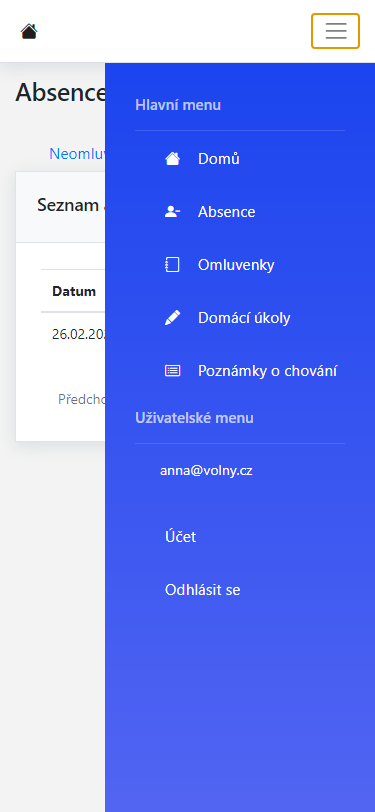
\includegraphics[width=0.5\textwidth]{images/aplikace_responzivni.png}
	\caption{Ukázka responzivního chování}
	\label{app-responz}
\end{figure}


\subsection{Výsledky testování}
Během testování bylo nalezeno několik menších, ale i závažnějších chyb. Menší chyby se týkaly především formulářů pro vyhledávání ve výsledcích, stránkování a responzivity. První závažnější chyba se objevila v administraci systému, kdy se při změně třídního učitele ve vybrané třídě vymazal původní třídní učitel z databáze. Chyba byla způsobena tím, že třídní učitel musel mít v databázi vyplněnou třídu, kterou má na starosti. Při změně třídního učitele tato podmínka nebyla splněna a uživatel byl ze systému vymazán. Další závažnější chyba se týkala opět administrace systému. Tentokrát se chyba objevila při změně rolí u zaměstnanců školy. Pokud se při přidání role \uv{třídní učitel} zapomnělo na vyplnění třídy, kde má uživatel vykonávat třídnické povinnosti, byl uživatel po potvrzení formuláře vymazán z databáze. Tato chyba byla způsobena především neošetřením formuláře na prázdné hodnoty a tím, že třídní učitel musel mít v databázi vyplněnou třídu, kterou má na starosti. Všechny menší i závažné chyby byly v systému opraveny.